%==============================================================================
% USGLoc -- Extended Report (companion to the RA-L letter usgloc_ral_draft.tex).
%
% Purpose: report EVERYTHING that does not fit the 6-page letter -- full
% implementation detail, the evidential-head (EDL) training analysis with
% measured numbers, map statistics, the retrieval-training study, extended
% result tables (per-scene calibration, full ablations, robustness, runtime),
% and the SGLoc-protocol comparison the letter cites as supplementary.
% This file doubles as the arXiv extended version / reviewer supplementary.
% Build: pdflatex -> bibtex -> pdflatex -> pdflatex (same toolchain as the letter).
%==============================================================================
\documentclass[journal]{IEEEtran}

\usepackage{amsmath,amssymb,amsfonts,bm}
\usepackage{graphicx}
\graphicspath{{figures/}}
\usepackage{xcolor}
\usepackage{booktabs}
\usepackage{cite}
\usepackage{url}
\usepackage{tikz}
\usetikzlibrary{positioning,arrows.meta,backgrounds,fit,calc}
\usepackage{orcidlink}
\usepackage[subpreambles=false]{standalone}

% ---- Shared colors for the \input'ed TikZ figures ----
\definecolor{ink}{HTML}{273746}
\definecolor{uLow}{HTML}{1B9E77}
\definecolor{uMid}{HTML}{E6AB02}
\definecolor{uHigh}{HTML}{D95F02}
\definecolor{coarseBg}{HTML}{EAF2FB}
\definecolor{coarseLn}{HTML}{9DC3EC}
\definecolor{fineBg}{HTML}{FDF1E6}
\definecolor{fineLn}{HTML}{F0C28E}
\definecolor{encBg}{HTML}{EEF6EE}
\definecolor{encLn}{HTML}{B7D8B7}
\definecolor{outBg}{HTML}{FFF3D6}
\definecolor{outLn}{HTML}{D9A300}
\definecolor{poseC}{HTML}{2E6FAC}
\definecolor{mapprin}{HTML}{E8F4EF}
\definecolor{mappt}{HTML}{F2F3F4}
\definecolor{locpt}{HTML}{EAF2FB}
\definecolor{ourstr}{HTML}{FFF3D6}

\newcommand{\res}{{\color{red}\textbf{--}}}
\newcommand{\TODO}[1]{{\color{red}[TODO: #1]}}
\newcommand{\figbox}[2]{%
  \fbox{\parbox[c][#1][c]{0.93\linewidth}{\centering\footnotesize #2}}}
\newcommand{\method}{USGLoc}

\begin{document}

\title{\method{}: Uncertainty-Aware Semantic Visual Localization from
3D Gaussian Splatting --- Extended Report}

\author{Thanh Nguyen Canh\orcidlink{0000-0001-6332-1002},~\IEEEmembership{Graduate Student Member,~IEEE},
Bang Nguyen Van, Xiem HoangVan, and Nak Young Chong\orcidlink{0000-0001-5736-0769},~\IEEEmembership{Senior Member,~IEEE}
\thanks{This work was supported by JST SPRING, Japan Grant Number JPMJSP2102.
(Corresponding authors: nakyoung@jaist.ac.jp, xiemhoang@vnu.edu.vn)}
\thanks{Thanh Nguyen Canh and Nak Young Chong are with the Japan Advanced
Institute of Science and Technology, Ishikawa 923-1211, Japan.}
\thanks{Bang Nguyen Van and Xiem HoangVan are with the University of
Engineering and Technology, Vietnam National University, Hanoi 10000, Vietnam.}}

\markboth{Extended report accompanying the RA-L submission}%
{Nguyen Canh \MakeLowercase{\textit{et al.}}: \method{} Extended Report}

\maketitle

%------------------------------------------------------------------------------
\begin{abstract}
This extended report accompanies the \method{} letter. The letter presents an
evidential localization framework on a 3D Gaussian Splatting (3DGS) map,
built on one principle: the map's own uncertainty should drive every stage of
localization and survive to the output. This report documents everything the
letter's page budget excludes. We give the complete implementation and
training recipes, an empirical analysis of the shared evidential head (EDL),
statistics of the evidential map, a study of retrieval-encoder training on
real data, per-scene calibration breakdowns, the full ablation grid, the
robustness sweeps, per-stage runtime, and the DSLAM-protocol comparison with
SGLoc referenced by the letter. Three implementation findings are reported
that we believe transfer to other evidential-perception systems:
(i) an EDL head's classification accuracy converges long before its
uncertainty structure does; (ii) a shared head must be trained on its full
deployment distribution --- both input domains AND all scenes --- or the
unseen part's evidence collapses; and (iii) viewpoint submaps must be
frustum-culled, or retrieval descriptors of a room-scale scene collapse onto
a single vector.
\end{abstract}

\begin{IEEEkeywords}
Localization, semantic scene understanding, uncertainty quantification,
evidential deep learning, Gaussian splatting.
\end{IEEEkeywords}

%------------------------------------------------------------------------------
\section{Scope and Relation to the Letter}
The RA-L letter (\emph{\method{}: Uncertainty-Aware Semantic Visual
Localization from 3D Gaussian Splatting}) is the primary publication: it
motivates the problem, derives the method (evidential map, vacuity-gated
matching, vacuity-weighted refinement, tempered Laplace posterior), and
reports the headline benchmark results. This report is the companion record.
Section~\ref{sec:impl} fixes every implementation detail. Sections
\ref{sec:edl}--\ref{sec:retrieval} analyze the three learned components with
measured numbers. Sections \ref{sec:protocol}--\ref{sec:sgloc} hold the
extended evaluation. Figure~1 of the letter (the pipeline overview) applies
unchanged and is reproduced in Fig.~\ref{fig:overview}.

\begin{figure*}[t]
  \centering
  \resizebox{\textwidth}{!}{% Fig. 1 -- USGLoc overview (standalone TikZ -> vector PDF).
% Compile standalone: pdflatex fig1_overview.tex
% In the paper: \resizebox{\textwidth}{!}{% Fig. 1 -- USGLoc overview (standalone TikZ -> vector PDF).
% Compile standalone: pdflatex fig1_overview.tex
% In the paper: \resizebox{\textwidth}{!}{% Fig. 1 -- USGLoc overview (standalone TikZ -> vector PDF).
% Compile standalone: pdflatex fig1_overview.tex
% In the paper: \resizebox{\textwidth}{!}{\input{figures/fig1_overview}}
%
% Design (after the STDLoc / UGS-Loc / GS-CPR / SplatHLoc figure study):
%  * slim grey OFFLINE strip (evidential mapping) on the left;
%  * Band A: the online pose flow (query -> matching -> hypotheses ->
%    refinement -> calibrated posterior);
%  * Band B: the EVIDENCE channel in gold underneath, injected upward into
%    Band A at four points (gate, correspondence gate, per-pixel weight,
%    temperature) -- the paper's thesis as the figure's macro-structure;
%  * every arrow carries an artifact glyph and a math symbol from the text;
%  * two accent colors only: gold = evidence, blue = pose distributions.
\documentclass[tikz,border=3pt]{standalone}
\usepackage{amsmath,amssymb,bm}
\usepackage{graphicx}
\usetikzlibrary{positioning,arrows.meta,backgrounds,fit,calc,shadings}

\definecolor{ink}{HTML}{273746}
\definecolor{uLow}{HTML}{1B9E77}
\definecolor{uMid}{HTML}{E6AB02}
\definecolor{uHigh}{HTML}{D95F02}
\definecolor{coarseBg}{HTML}{EAF2FB}
\definecolor{coarseLn}{HTML}{9DC3EC}
\definecolor{fineBg}{HTML}{FDF1E6}
\definecolor{fineLn}{HTML}{F0C28E}
\definecolor{encBg}{HTML}{EEF6EE}
\definecolor{encLn}{HTML}{B7D8B7}
\definecolor{outBg}{HTML}{FFF3D6}
\definecolor{outLn}{HTML}{D9A300}
\definecolor{poseC}{HTML}{2E6FAC}

\begin{document}
\begin{tikzpicture}[
  font=\footnotesize\color{ink},
  >={Stealth[length=2mm]},
  mod/.style={draw=ink!75, fill=white, rounded corners=2pt, align=center,
              minimum height=10mm, inner sep=2.5pt, line width=0.5pt},
  flow/.style={->, line width=0.7pt, draw=ink!80},
  evflow/.style={->, line width=1.0pt, draw=outLn},
  inject/.style={->, line width=1.0pt, draw=outLn, dashed},
  sym/.style={font=\scriptsize\color{ink}, inner sep=1.5pt, fill=white,
              fill opacity=0.85, text opacity=1},
  sub/.style={font=\scriptsize\color{ink!75}, align=center},
  panlab/.style={font=\scriptsize\bfseries\color{ink!80}}
]

% ============================ OFFLINE STRIP =================================
% mapping frames: three real training views
\foreach \i/\dx/\dy in {2/0.16/0.16, 1/0.08/0.08, 0/0/0}{
  \node[inner sep=0pt, draw=ink!60, line width=0.35pt]
    at (1.15+\dx, 1.42+\dy) {\includegraphics[width=10mm]{fig1_blocks/mapframe\i.png}};
}
\node[sub, anchor=north] at (1.15, 0.92) {mapping frames};
\draw[flow] (1.15, 0.72) -- (1.15, 0.12);
\node[mod, text width=23mm, font=\scriptsize\color{ink}] (edlhead) at (1.15,-0.42)
  {semantic 3DGS\\ + EDL head (3)};
\draw[flow] (1.15,-0.98) -- node[sym, right=0mm] {$(\mathbf{b},u)$} (1.15,-1.22);
% evidential map: splats colored by vacuity
% the real map, rendered from a free camera: Gaussians, not a schematic
\node[inner sep=0pt, draw=ink!60, line width=0.35pt] (map3d) at (1.15,-2.00)
  {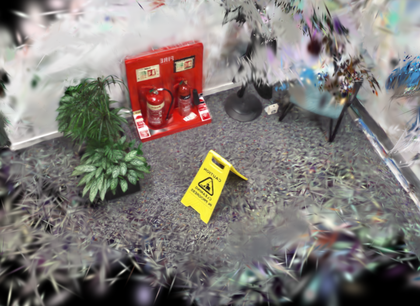
\includegraphics[width=20mm]{fig1_blocks/map3d.png}};
% vacuity key, so the colour channel carried below means something
\foreach \i/\c in {0/uLow, 1/uMid, 2/uHigh}{
  \shade[inner color=\c!25, outer color=\c!85] (0.42+0.26*\i, -3.00) circle (0.9mm);
}
\node[sub, anchor=west, font=\tiny\color{ink!75}] at (1.08,-3.00) {$u$: low$\to$high};
\node[sub, anchor=north, text width=30mm] at (1.15,-3.18)
  {evidential map $\mathcal{M}{=}\{\mathcal{G}_i\}$\\[-0.4mm]
   {\tiny $\mathcal{G}_i{=}(\bm\mu_i,\bm\Sigma_i,f_i,\mathbf{p}_i,\tilde u_i)$}};

% ============================== BAND A ======================================
% query
\node[inner sep=0pt, draw=ink!70, line width=0.5pt] (qimg) at (3.92, 1.01)
  {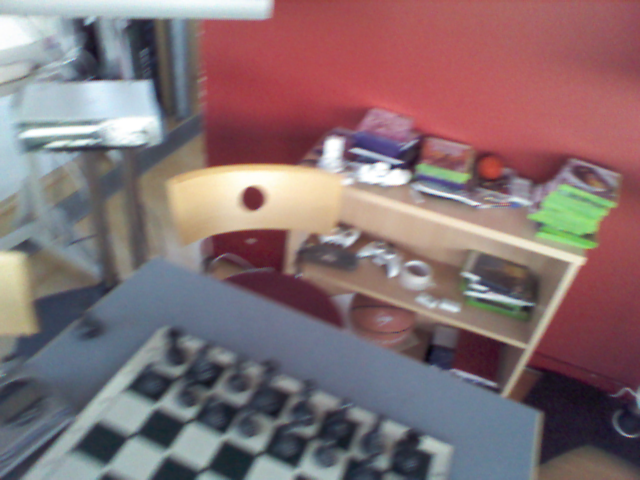
\includegraphics[width=11.5mm]{fig4/a_query.png}};
\node[sub, anchor=north] at (3.92, 0.55) {query $I_q$};

% evidential encoding
\node[mod, text width=25mm] (enc) at (6.05, 1.0)
  {Evidential\\encoding (III-B)\\{\scriptsize $\mathcal{Q}_j{=}(\mathbf{x},a,f^q,\mathbf{p}^q,u^q)$}};
\draw[flow] (4.5, 1.0) -- (enc.west);

% gated matching, with match-line glyph showing gating
\node[mod, text width=24mm, minimum height=13mm] (match) at (9.35, 1.0)
  {Vacuity-gated\\matching (III-C)};
\draw[flow] (enc.east) -- node[sym, above=0mm] {$d^q_j$} (match.west);
% match glyph below the box: two frames, kept (green) and gated-out (orange) matches
\begin{scope}[shift={(8.55, 0.28)}]
  \draw[ink!55, line width=0.4pt] (0,0) rectangle +(0.5,0.36);
  \draw[ink!55, line width=0.4pt] (1.1,0) rectangle +(0.5,0.36);
  \draw[uLow, line width=0.5pt]  (0.5,0.28) -- (1.1,0.30);
  \draw[uLow, line width=0.5pt]  (0.5,0.16) -- (1.1,0.12);
  \draw[uHigh, line width=0.5pt, dash pattern=on 1pt off 1pt] (0.5,0.05) -- (1.1,0.22);
\end{scope}

% top-k hypotheses: three fading camera frusta
\begin{scope}[shift={(12.15, 0.72)}]
  \foreach \dx/\op in {0/0.9, 0.42/0.55, 0.84/0.3}{
    \begin{scope}[shift={(\dx,0)}, opacity=\op]
      \fill[poseC!25] (0,0.66) -- (0,0.10) -- (0.5,0.38) -- cycle;
      \draw[poseC, line width=0.6pt] (0,0.66) -- (0,0.10) -- (0.5,0.38) -- cycle;
    \end{scope}
  }
\end{scope}
\node[sub, anchor=north, text width=24mm] (hyplab) at (12.85, 0.62)
  {top-$k$ hypotheses\\$\{(T^0_k,\tilde\pi_k)\}$};
\draw[flow] (match.east) -- node[sym, above=0mm] {$s_{ij}$ (6)} (12.0, 1.0);

% ---- row 2 (correction + fine + pose head), shifted under row 1 ----------
\node[mod, text width=24mm, minimum height=13mm] (corr) at (3.50, -5.80)
  {Matching\\correction (III-D)\\{\scriptsize PnP on gated matches (8)}};
\node[mod, text width=26mm, minimum height=13mm] (refine) at (6.75, -5.80)
  {Vacuity-weighted\\refinement (III-E)\\{\scriptsize $E(\bm{\xi})$ (10)}};
\node[inner sep=0pt, draw=ink!55, line width=0.4pt] (wimg) at (6.75,-7.15)
  {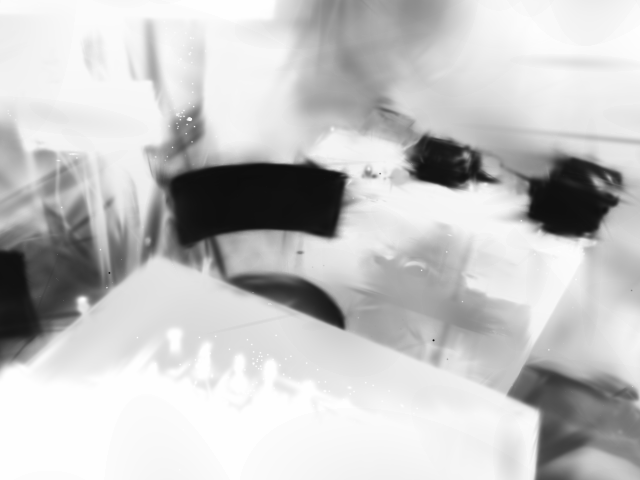
\includegraphics[width=12mm]{fig4/a_weight.png}};
\node[sub, anchor=north] at (6.75,-7.58) {per-pixel weight $w$};
\draw[flow] (corr.east) -- node[sym, above=0mm] {$T'_k$} (refine.west);

% ---- calibrated pose head ----
\node[mod, text width=21mm] (lap) at (10.15, -5.80)
  {Laplace cov.\ (11)\\{\scriptsize $\bm{\Sigma}_{\bm{\xi},k}\!\leftarrow\!\tau\hat\sigma^2(J^{\!\top}\!WJ)^{-1}$}};
\draw[flow] (refine.east) -- node[sym, above=0mm] {$\bm{\xi}^\star_k$} (lap.west);
% GMM glyph: overlapping covariance ellipses
\begin{scope}[shift={(12.55, -5.98)}]
  \draw[poseC!85, line width=0.6pt, rotate around={18:(0.32,0.28)}]
    (0.32,0.28) ellipse (4.6mm and 2.4mm);
  \draw[poseC!85, line width=0.6pt, rotate around={-12:(0.95,0.46)}]
    (0.95,0.46) ellipse (3.2mm and 1.8mm);
  \fill[poseC] (0.32,0.28) circle (0.5pt);
  \fill[poseC] (0.95,0.46) circle (0.5pt);
\end{scope}
\node[sub, anchor=north, text width=26mm] at (13.20, -6.25)
  {$p(T|I_q,\mathcal{M})$ (12)\\condense $\rightarrow$ EKF};
\draw[flow] (lap.east) -- (11.95, -5.80);

% ---- the serpentine turn: row 1 ends, row 2 begins -----------------------
\draw[flow] (13.85, 1.0) -- (14.75, 1.0) -- (14.75, -4.12)
            -- (1.30, -4.12) -- (1.30, -5.80) -- (corr.west);


% ============================== BAND B ======================================
% opinion simplex glyph
\begin{scope}[shift={(5.55,-2.65)}]
  \draw[outLn, line width=0.6pt] (0,0) -- (1.0,0) -- (0.5,0.8) -- cycle;
  \fill[outLn!45] (0.42,0.30) circle (1.6mm);
  \node[sub, anchor=north] at (0.5,-0.08) {opinion $(\mathbf{b},u)$};
\end{scope}
% DST fusion glyph: two small simplexes -> one
\begin{scope}[shift={(8.55,-2.45)}]
  \draw[outLn!70, line width=0.5pt] (0,0.12) -- (0.44,0.12) -- (0.22,0.48) -- cycle;
  \draw[outLn!70, line width=0.5pt] (0,-0.42) -- (0.44,-0.42) -- (0.22,-0.06) -- cycle;
  \node[font=\scriptsize\color{outLn}] at (0.68,-0.02) {$\oplus$};
  \draw[outLn, line width=0.6pt] (0.9,-0.28) -- (1.5,-0.28) -- (1.2,0.22) -- cycle;
  \node[sub, anchor=north, text width=24mm] at (0.26,-0.56)
    {conflict-aware fusion (4)\\[-0.3mm]{\tiny $\tilde{u}{=}\min(1,u{+}\bar\eta)$}};
\end{scope}
% vacuity heatmap glyph U_r
\node[inner sep=0pt, draw=ink!55, line width=0.4pt] (urimg) at (10.95,-2.34)
  {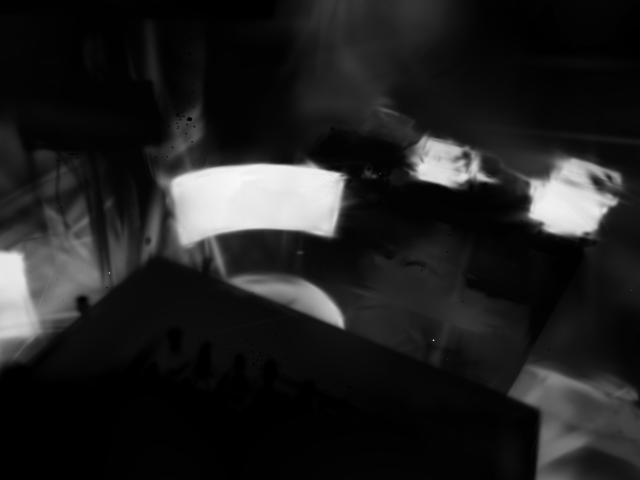
\includegraphics[width=12mm]{fig4/a_vacuity.png}};
\node[sub, anchor=north] at (11.05,-2.90) {rendered $U_r$ (9)};
% temperature chip
\node[mod, draw=outLn, text width=16mm, font=\scriptsize\color{ink}] (temp) at (13.35,-2.45)
  {temperature $\tau$\\(held-out fit)};

% the gold evidence rail
\draw[evflow] (2.1,-2.1) -- node[sym, above=0mm] {$u$} (5.45,-2.35);
\draw[evflow] (6.75,-2.35) -- (8.4,-2.5);
\draw[evflow] (9.95,-2.34) -- node[sym, above=0.6mm, pos=0.45] {$\tilde{u}_i$ per splat} (urimg.west);
\draw[evflow] (urimg.east) -- (temp.west);

% injections: UP into row 1, DOWN into row 2 -- one channel, both bands
\draw[inject] (9.35,-1.95) -- node[sym, right=0.2mm]
  {gate $e^{-\lambda_u(\tilde{u}^G_i+u^q_j)}$} (match.south);
\draw[inject] (10.25,-3.60) -- node[sym, left=0.2mm, pos=0.42, fill=white, inner sep=1pt]
  {$\bar U_r{\le}u_{\max}$} (corr.north);
\draw[inject] (11.65,-3.60) -- node[sym, right=0.2mm, pos=0.42, fill=white, inner sep=1pt]
  {$w{=}e^{-\gamma U_r}$} (refine.north);
\draw[inject] (temp.south) -- node[sym, right=0.2mm] {$\tau$} (lap.north);

% ======================= PANELS (background layer) ==========================
\begin{scope}[on background layer]
  % offline strip
  \node[fill=ink!5, draw=ink!35, dashed, rounded corners=3pt, inner sep=2.6mm,
        fit={(edlhead) (map3d) (-0.20,2.05) (2.55,-3.95)}] (offpan) {};
  % coarse panel
  \node[fill=coarseBg, draw=coarseLn, rounded corners=3pt, inner sep=2.8mm,
        fit={(enc) (match) (hyplab) (13.9,0.2)}] (cpan) {};
  % fine panel
  \node[fill=fineBg, draw=fineLn, rounded corners=3pt, inner sep=2.8mm,
        fit={(corr) (refine) (wimg) (6.75,-7.75)}] (fpan) {};
  % calibrated pose head panel
  \node[fill=poseC!8, draw=poseC!60, rounded corners=3pt, inner sep=2.8mm,
        fit={(lap) (14.6,-6.45) (14.6,-5.25)}] (ppan) {};
  % evidence band
  \node[fill=outBg, draw=outLn!70, rounded corners=3pt, inner sep=2.8mm,
        fit={(5.45,-1.8) (temp) (urimg) (14.3,-3.42) (5.45,-3.42)}] (epan) {};
\end{scope}
\node[panlab, anchor=south west] at (offpan.north west)
  {Offline: evidential mapping (III-A)};
\node[panlab, anchor=south west] at (cpan.north west) {Coarse (IV-B,C)};
\node[panlab, anchor=south west] at (fpan.north west) {Correction + fine (IV-D,E)};
\node[panlab, anchor=south west, color=poseC] at (ppan.north west)
  {Calibrated pose posterior};
\node[panlab, anchor=south west, color=outLn!80!ink] at (epan.north west)
  {One evidential channel: created once, never dropped};

% map feeds the online flow
\draw[flow] (2.18,-0.42) -- node[sym, above=0.4mm, pos=0.62] {$\mathcal{M}$}
  (2.95,-0.42) -- (8.4,-0.42) -- (match.south west);

\end{tikzpicture}
\end{document}
}
%
% Design (after the STDLoc / UGS-Loc / GS-CPR / SplatHLoc figure study):
%  * slim grey OFFLINE strip (evidential mapping) on the left;
%  * Band A: the online pose flow (query -> matching -> hypotheses ->
%    refinement -> calibrated posterior);
%  * Band B: the EVIDENCE channel in gold underneath, injected upward into
%    Band A at four points (gate, correspondence gate, per-pixel weight,
%    temperature) -- the paper's thesis as the figure's macro-structure;
%  * every arrow carries an artifact glyph and a math symbol from the text;
%  * two accent colors only: gold = evidence, blue = pose distributions.
\documentclass[tikz,border=3pt]{standalone}
\usepackage{amsmath,amssymb,bm}
\usepackage{graphicx}
\usetikzlibrary{positioning,arrows.meta,backgrounds,fit,calc,shadings}

\definecolor{ink}{HTML}{273746}
\definecolor{uLow}{HTML}{1B9E77}
\definecolor{uMid}{HTML}{E6AB02}
\definecolor{uHigh}{HTML}{D95F02}
\definecolor{coarseBg}{HTML}{EAF2FB}
\definecolor{coarseLn}{HTML}{9DC3EC}
\definecolor{fineBg}{HTML}{FDF1E6}
\definecolor{fineLn}{HTML}{F0C28E}
\definecolor{encBg}{HTML}{EEF6EE}
\definecolor{encLn}{HTML}{B7D8B7}
\definecolor{outBg}{HTML}{FFF3D6}
\definecolor{outLn}{HTML}{D9A300}
\definecolor{poseC}{HTML}{2E6FAC}

\begin{document}
\begin{tikzpicture}[
  font=\footnotesize\color{ink},
  >={Stealth[length=2mm]},
  mod/.style={draw=ink!75, fill=white, rounded corners=2pt, align=center,
              minimum height=10mm, inner sep=2.5pt, line width=0.5pt},
  flow/.style={->, line width=0.7pt, draw=ink!80},
  evflow/.style={->, line width=1.0pt, draw=outLn},
  inject/.style={->, line width=1.0pt, draw=outLn, dashed},
  sym/.style={font=\scriptsize\color{ink}, inner sep=1.5pt, fill=white,
              fill opacity=0.85, text opacity=1},
  sub/.style={font=\scriptsize\color{ink!75}, align=center},
  panlab/.style={font=\scriptsize\bfseries\color{ink!80}}
]

% ============================ OFFLINE STRIP =================================
% mapping frames: three real training views
\foreach \i/\dx/\dy in {2/0.16/0.16, 1/0.08/0.08, 0/0/0}{
  \node[inner sep=0pt, draw=ink!60, line width=0.35pt]
    at (1.15+\dx, 1.42+\dy) {\includegraphics[width=10mm]{fig1_blocks/mapframe\i.png}};
}
\node[sub, anchor=north] at (1.15, 0.92) {mapping frames};
\draw[flow] (1.15, 0.72) -- (1.15, 0.12);
\node[mod, text width=23mm, font=\scriptsize\color{ink}] (edlhead) at (1.15,-0.42)
  {semantic 3DGS\\ + EDL head (3)};
\draw[flow] (1.15,-0.98) -- node[sym, right=0mm] {$(\mathbf{b},u)$} (1.15,-1.22);
% evidential map: splats colored by vacuity
% the real map, rendered from a free camera: Gaussians, not a schematic
\node[inner sep=0pt, draw=ink!60, line width=0.35pt] (map3d) at (1.15,-2.00)
  {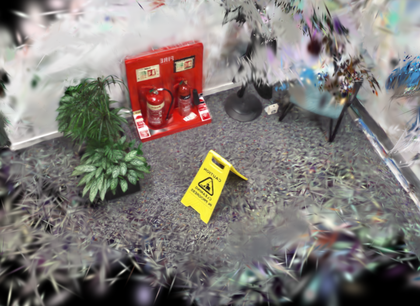
\includegraphics[width=20mm]{fig1_blocks/map3d.png}};
% vacuity key, so the colour channel carried below means something
\foreach \i/\c in {0/uLow, 1/uMid, 2/uHigh}{
  \shade[inner color=\c!25, outer color=\c!85] (0.42+0.26*\i, -3.00) circle (0.9mm);
}
\node[sub, anchor=west, font=\tiny\color{ink!75}] at (1.08,-3.00) {$u$: low$\to$high};
\node[sub, anchor=north, text width=30mm] at (1.15,-3.18)
  {evidential map $\mathcal{M}{=}\{\mathcal{G}_i\}$\\[-0.4mm]
   {\tiny $\mathcal{G}_i{=}(\bm\mu_i,\bm\Sigma_i,f_i,\mathbf{p}_i,\tilde u_i)$}};

% ============================== BAND A ======================================
% query
\node[inner sep=0pt, draw=ink!70, line width=0.5pt] (qimg) at (3.92, 1.01)
  {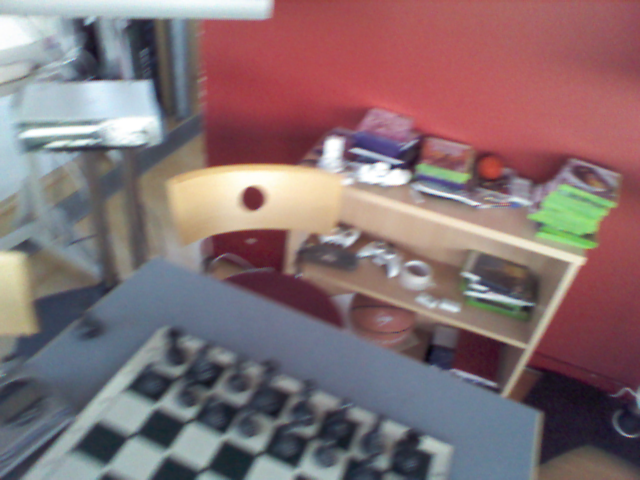
\includegraphics[width=11.5mm]{fig4/a_query.png}};
\node[sub, anchor=north] at (3.92, 0.55) {query $I_q$};

% evidential encoding
\node[mod, text width=25mm] (enc) at (6.05, 1.0)
  {Evidential\\encoding (III-B)\\{\scriptsize $\mathcal{Q}_j{=}(\mathbf{x},a,f^q,\mathbf{p}^q,u^q)$}};
\draw[flow] (4.5, 1.0) -- (enc.west);

% gated matching, with match-line glyph showing gating
\node[mod, text width=24mm, minimum height=13mm] (match) at (9.35, 1.0)
  {Vacuity-gated\\matching (III-C)};
\draw[flow] (enc.east) -- node[sym, above=0mm] {$d^q_j$} (match.west);
% match glyph below the box: two frames, kept (green) and gated-out (orange) matches
\begin{scope}[shift={(8.55, 0.28)}]
  \draw[ink!55, line width=0.4pt] (0,0) rectangle +(0.5,0.36);
  \draw[ink!55, line width=0.4pt] (1.1,0) rectangle +(0.5,0.36);
  \draw[uLow, line width=0.5pt]  (0.5,0.28) -- (1.1,0.30);
  \draw[uLow, line width=0.5pt]  (0.5,0.16) -- (1.1,0.12);
  \draw[uHigh, line width=0.5pt, dash pattern=on 1pt off 1pt] (0.5,0.05) -- (1.1,0.22);
\end{scope}

% top-k hypotheses: three fading camera frusta
\begin{scope}[shift={(12.15, 0.72)}]
  \foreach \dx/\op in {0/0.9, 0.42/0.55, 0.84/0.3}{
    \begin{scope}[shift={(\dx,0)}, opacity=\op]
      \fill[poseC!25] (0,0.66) -- (0,0.10) -- (0.5,0.38) -- cycle;
      \draw[poseC, line width=0.6pt] (0,0.66) -- (0,0.10) -- (0.5,0.38) -- cycle;
    \end{scope}
  }
\end{scope}
\node[sub, anchor=north, text width=24mm] (hyplab) at (12.85, 0.62)
  {top-$k$ hypotheses\\$\{(T^0_k,\tilde\pi_k)\}$};
\draw[flow] (match.east) -- node[sym, above=0mm] {$s_{ij}$ (6)} (12.0, 1.0);

% ---- row 2 (correction + fine + pose head), shifted under row 1 ----------
\node[mod, text width=24mm, minimum height=13mm] (corr) at (3.50, -5.80)
  {Matching\\correction (III-D)\\{\scriptsize PnP on gated matches (8)}};
\node[mod, text width=26mm, minimum height=13mm] (refine) at (6.75, -5.80)
  {Vacuity-weighted\\refinement (III-E)\\{\scriptsize $E(\bm{\xi})$ (10)}};
\node[inner sep=0pt, draw=ink!55, line width=0.4pt] (wimg) at (6.75,-7.15)
  {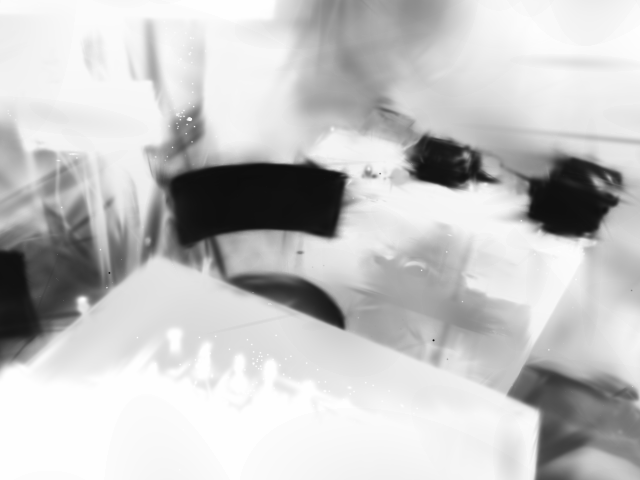
\includegraphics[width=12mm]{fig4/a_weight.png}};
\node[sub, anchor=north] at (6.75,-7.58) {per-pixel weight $w$};
\draw[flow] (corr.east) -- node[sym, above=0mm] {$T'_k$} (refine.west);

% ---- calibrated pose head ----
\node[mod, text width=21mm] (lap) at (10.15, -5.80)
  {Laplace cov.\ (11)\\{\scriptsize $\bm{\Sigma}_{\bm{\xi},k}\!\leftarrow\!\tau\hat\sigma^2(J^{\!\top}\!WJ)^{-1}$}};
\draw[flow] (refine.east) -- node[sym, above=0mm] {$\bm{\xi}^\star_k$} (lap.west);
% GMM glyph: overlapping covariance ellipses
\begin{scope}[shift={(12.55, -5.98)}]
  \draw[poseC!85, line width=0.6pt, rotate around={18:(0.32,0.28)}]
    (0.32,0.28) ellipse (4.6mm and 2.4mm);
  \draw[poseC!85, line width=0.6pt, rotate around={-12:(0.95,0.46)}]
    (0.95,0.46) ellipse (3.2mm and 1.8mm);
  \fill[poseC] (0.32,0.28) circle (0.5pt);
  \fill[poseC] (0.95,0.46) circle (0.5pt);
\end{scope}
\node[sub, anchor=north, text width=26mm] at (13.20, -6.25)
  {$p(T|I_q,\mathcal{M})$ (12)\\condense $\rightarrow$ EKF};
\draw[flow] (lap.east) -- (11.95, -5.80);

% ---- the serpentine turn: row 1 ends, row 2 begins -----------------------
\draw[flow] (13.85, 1.0) -- (14.75, 1.0) -- (14.75, -4.12)
            -- (1.30, -4.12) -- (1.30, -5.80) -- (corr.west);


% ============================== BAND B ======================================
% opinion simplex glyph
\begin{scope}[shift={(5.55,-2.65)}]
  \draw[outLn, line width=0.6pt] (0,0) -- (1.0,0) -- (0.5,0.8) -- cycle;
  \fill[outLn!45] (0.42,0.30) circle (1.6mm);
  \node[sub, anchor=north] at (0.5,-0.08) {opinion $(\mathbf{b},u)$};
\end{scope}
% DST fusion glyph: two small simplexes -> one
\begin{scope}[shift={(8.55,-2.45)}]
  \draw[outLn!70, line width=0.5pt] (0,0.12) -- (0.44,0.12) -- (0.22,0.48) -- cycle;
  \draw[outLn!70, line width=0.5pt] (0,-0.42) -- (0.44,-0.42) -- (0.22,-0.06) -- cycle;
  \node[font=\scriptsize\color{outLn}] at (0.68,-0.02) {$\oplus$};
  \draw[outLn, line width=0.6pt] (0.9,-0.28) -- (1.5,-0.28) -- (1.2,0.22) -- cycle;
  \node[sub, anchor=north, text width=24mm] at (0.26,-0.56)
    {conflict-aware fusion (4)\\[-0.3mm]{\tiny $\tilde{u}{=}\min(1,u{+}\bar\eta)$}};
\end{scope}
% vacuity heatmap glyph U_r
\node[inner sep=0pt, draw=ink!55, line width=0.4pt] (urimg) at (10.95,-2.34)
  {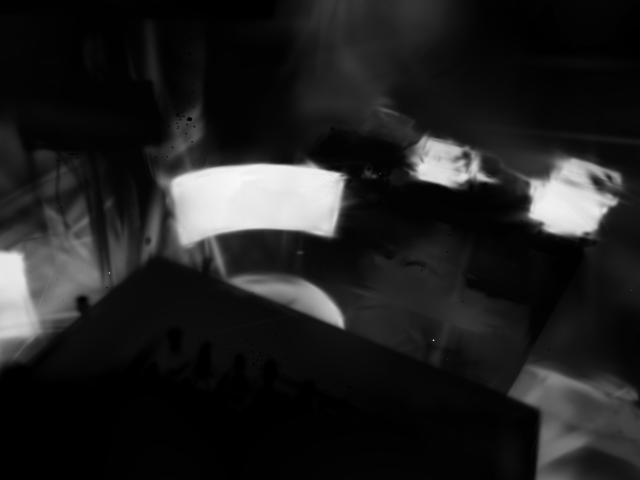
\includegraphics[width=12mm]{fig4/a_vacuity.png}};
\node[sub, anchor=north] at (11.05,-2.90) {rendered $U_r$ (9)};
% temperature chip
\node[mod, draw=outLn, text width=16mm, font=\scriptsize\color{ink}] (temp) at (13.35,-2.45)
  {temperature $\tau$\\(held-out fit)};

% the gold evidence rail
\draw[evflow] (2.1,-2.1) -- node[sym, above=0mm] {$u$} (5.45,-2.35);
\draw[evflow] (6.75,-2.35) -- (8.4,-2.5);
\draw[evflow] (9.95,-2.34) -- node[sym, above=0.6mm, pos=0.45] {$\tilde{u}_i$ per splat} (urimg.west);
\draw[evflow] (urimg.east) -- (temp.west);

% injections: UP into row 1, DOWN into row 2 -- one channel, both bands
\draw[inject] (9.35,-1.95) -- node[sym, right=0.2mm]
  {gate $e^{-\lambda_u(\tilde{u}^G_i+u^q_j)}$} (match.south);
\draw[inject] (10.25,-3.60) -- node[sym, left=0.2mm, pos=0.42, fill=white, inner sep=1pt]
  {$\bar U_r{\le}u_{\max}$} (corr.north);
\draw[inject] (11.65,-3.60) -- node[sym, right=0.2mm, pos=0.42, fill=white, inner sep=1pt]
  {$w{=}e^{-\gamma U_r}$} (refine.north);
\draw[inject] (temp.south) -- node[sym, right=0.2mm] {$\tau$} (lap.north);

% ======================= PANELS (background layer) ==========================
\begin{scope}[on background layer]
  % offline strip
  \node[fill=ink!5, draw=ink!35, dashed, rounded corners=3pt, inner sep=2.6mm,
        fit={(edlhead) (map3d) (-0.20,2.05) (2.55,-3.95)}] (offpan) {};
  % coarse panel
  \node[fill=coarseBg, draw=coarseLn, rounded corners=3pt, inner sep=2.8mm,
        fit={(enc) (match) (hyplab) (13.9,0.2)}] (cpan) {};
  % fine panel
  \node[fill=fineBg, draw=fineLn, rounded corners=3pt, inner sep=2.8mm,
        fit={(corr) (refine) (wimg) (6.75,-7.75)}] (fpan) {};
  % calibrated pose head panel
  \node[fill=poseC!8, draw=poseC!60, rounded corners=3pt, inner sep=2.8mm,
        fit={(lap) (14.6,-6.45) (14.6,-5.25)}] (ppan) {};
  % evidence band
  \node[fill=outBg, draw=outLn!70, rounded corners=3pt, inner sep=2.8mm,
        fit={(5.45,-1.8) (temp) (urimg) (14.3,-3.42) (5.45,-3.42)}] (epan) {};
\end{scope}
\node[panlab, anchor=south west] at (offpan.north west)
  {Offline: evidential mapping (III-A)};
\node[panlab, anchor=south west] at (cpan.north west) {Coarse (IV-B,C)};
\node[panlab, anchor=south west] at (fpan.north west) {Correction + fine (IV-D,E)};
\node[panlab, anchor=south west, color=poseC] at (ppan.north west)
  {Calibrated pose posterior};
\node[panlab, anchor=south west, color=outLn!80!ink] at (epan.north west)
  {One evidential channel: created once, never dropped};

% map feeds the online flow
\draw[flow] (2.18,-0.42) -- node[sym, above=0.4mm, pos=0.62] {$\mathcal{M}$}
  (2.95,-0.42) -- (8.4,-0.42) -- (match.south west);

\end{tikzpicture}
\end{document}
}
%
% Design (after the STDLoc / UGS-Loc / GS-CPR / SplatHLoc figure study):
%  * slim grey OFFLINE strip (evidential mapping) on the left;
%  * Band A: the online pose flow (query -> matching -> hypotheses ->
%    refinement -> calibrated posterior);
%  * Band B: the EVIDENCE channel in gold underneath, injected upward into
%    Band A at four points (gate, correspondence gate, per-pixel weight,
%    temperature) -- the paper's thesis as the figure's macro-structure;
%  * every arrow carries an artifact glyph and a math symbol from the text;
%  * two accent colors only: gold = evidence, blue = pose distributions.
\documentclass[tikz,border=3pt]{standalone}
\usepackage{amsmath,amssymb,bm}
\usepackage{graphicx}
\usetikzlibrary{positioning,arrows.meta,backgrounds,fit,calc,shadings}

\definecolor{ink}{HTML}{273746}
\definecolor{uLow}{HTML}{1B9E77}
\definecolor{uMid}{HTML}{E6AB02}
\definecolor{uHigh}{HTML}{D95F02}
\definecolor{coarseBg}{HTML}{EAF2FB}
\definecolor{coarseLn}{HTML}{9DC3EC}
\definecolor{fineBg}{HTML}{FDF1E6}
\definecolor{fineLn}{HTML}{F0C28E}
\definecolor{encBg}{HTML}{EEF6EE}
\definecolor{encLn}{HTML}{B7D8B7}
\definecolor{outBg}{HTML}{FFF3D6}
\definecolor{outLn}{HTML}{D9A300}
\definecolor{poseC}{HTML}{2E6FAC}

\begin{document}
\begin{tikzpicture}[
  font=\footnotesize\color{ink},
  >={Stealth[length=2mm]},
  mod/.style={draw=ink!75, fill=white, rounded corners=2pt, align=center,
              minimum height=10mm, inner sep=2.5pt, line width=0.5pt},
  flow/.style={->, line width=0.7pt, draw=ink!80},
  evflow/.style={->, line width=1.0pt, draw=outLn},
  inject/.style={->, line width=1.0pt, draw=outLn, dashed},
  sym/.style={font=\scriptsize\color{ink}, inner sep=1.5pt, fill=white,
              fill opacity=0.85, text opacity=1},
  sub/.style={font=\scriptsize\color{ink!75}, align=center},
  panlab/.style={font=\scriptsize\bfseries\color{ink!80}}
]

% ============================ OFFLINE STRIP =================================
% mapping frames: three real training views
\foreach \i/\dx/\dy in {2/0.16/0.16, 1/0.08/0.08, 0/0/0}{
  \node[inner sep=0pt, draw=ink!60, line width=0.35pt]
    at (1.15+\dx, 1.42+\dy) {\includegraphics[width=10mm]{fig1_blocks/mapframe\i.png}};
}
\node[sub, anchor=north] at (1.15, 0.92) {mapping frames};
\draw[flow] (1.15, 0.72) -- (1.15, 0.12);
\node[mod, text width=23mm, font=\scriptsize\color{ink}] (edlhead) at (1.15,-0.42)
  {semantic 3DGS\\ + EDL head (3)};
\draw[flow] (1.15,-0.98) -- node[sym, right=0mm] {$(\mathbf{b},u)$} (1.15,-1.22);
% evidential map: splats colored by vacuity
% the real map, rendered from a free camera: Gaussians, not a schematic
\node[inner sep=0pt, draw=ink!60, line width=0.35pt] (map3d) at (1.15,-2.00)
  {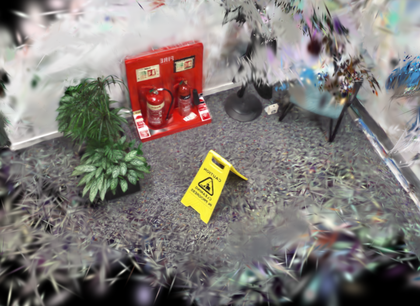
\includegraphics[width=20mm]{fig1_blocks/map3d.png}};
% vacuity key, so the colour channel carried below means something
\foreach \i/\c in {0/uLow, 1/uMid, 2/uHigh}{
  \shade[inner color=\c!25, outer color=\c!85] (0.42+0.26*\i, -3.00) circle (0.9mm);
}
\node[sub, anchor=west, font=\tiny\color{ink!75}] at (1.08,-3.00) {$u$: low$\to$high};
\node[sub, anchor=north, text width=30mm] at (1.15,-3.18)
  {evidential map $\mathcal{M}{=}\{\mathcal{G}_i\}$\\[-0.4mm]
   {\tiny $\mathcal{G}_i{=}(\bm\mu_i,\bm\Sigma_i,f_i,\mathbf{p}_i,\tilde u_i)$}};

% ============================== BAND A ======================================
% query
\node[inner sep=0pt, draw=ink!70, line width=0.5pt] (qimg) at (3.92, 1.01)
  {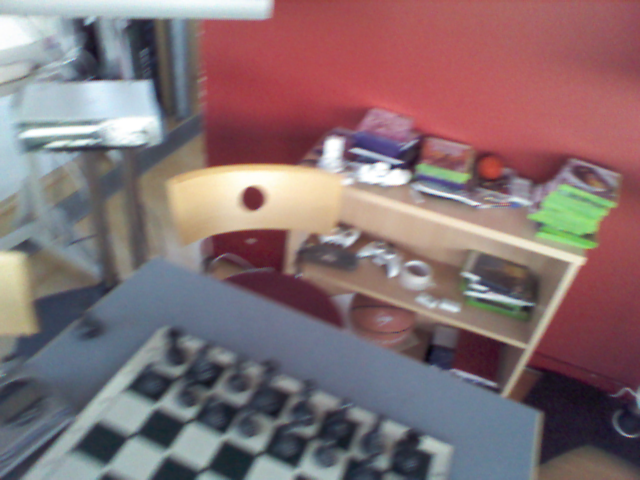
\includegraphics[width=11.5mm]{fig4/a_query.png}};
\node[sub, anchor=north] at (3.92, 0.55) {query $I_q$};

% evidential encoding
\node[mod, text width=25mm] (enc) at (6.05, 1.0)
  {Evidential\\encoding (III-B)\\{\scriptsize $\mathcal{Q}_j{=}(\mathbf{x},a,f^q,\mathbf{p}^q,u^q)$}};
\draw[flow] (4.5, 1.0) -- (enc.west);

% gated matching, with match-line glyph showing gating
\node[mod, text width=24mm, minimum height=13mm] (match) at (9.35, 1.0)
  {Vacuity-gated\\matching (III-C)};
\draw[flow] (enc.east) -- node[sym, above=0mm] {$d^q_j$} (match.west);
% match glyph below the box: two frames, kept (green) and gated-out (orange) matches
\begin{scope}[shift={(8.55, 0.28)}]
  \draw[ink!55, line width=0.4pt] (0,0) rectangle +(0.5,0.36);
  \draw[ink!55, line width=0.4pt] (1.1,0) rectangle +(0.5,0.36);
  \draw[uLow, line width=0.5pt]  (0.5,0.28) -- (1.1,0.30);
  \draw[uLow, line width=0.5pt]  (0.5,0.16) -- (1.1,0.12);
  \draw[uHigh, line width=0.5pt, dash pattern=on 1pt off 1pt] (0.5,0.05) -- (1.1,0.22);
\end{scope}

% top-k hypotheses: three fading camera frusta
\begin{scope}[shift={(12.15, 0.72)}]
  \foreach \dx/\op in {0/0.9, 0.42/0.55, 0.84/0.3}{
    \begin{scope}[shift={(\dx,0)}, opacity=\op]
      \fill[poseC!25] (0,0.66) -- (0,0.10) -- (0.5,0.38) -- cycle;
      \draw[poseC, line width=0.6pt] (0,0.66) -- (0,0.10) -- (0.5,0.38) -- cycle;
    \end{scope}
  }
\end{scope}
\node[sub, anchor=north, text width=24mm] (hyplab) at (12.85, 0.62)
  {top-$k$ hypotheses\\$\{(T^0_k,\tilde\pi_k)\}$};
\draw[flow] (match.east) -- node[sym, above=0mm] {$s_{ij}$ (6)} (12.0, 1.0);

% ---- row 2 (correction + fine + pose head), shifted under row 1 ----------
\node[mod, text width=24mm, minimum height=13mm] (corr) at (3.50, -5.80)
  {Matching\\correction (III-D)\\{\scriptsize PnP on gated matches (8)}};
\node[mod, text width=26mm, minimum height=13mm] (refine) at (6.75, -5.80)
  {Vacuity-weighted\\refinement (III-E)\\{\scriptsize $E(\bm{\xi})$ (10)}};
\node[inner sep=0pt, draw=ink!55, line width=0.4pt] (wimg) at (6.75,-7.15)
  {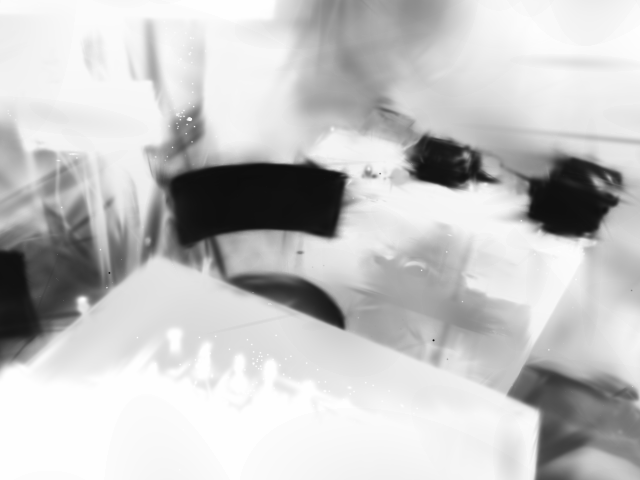
\includegraphics[width=12mm]{fig4/a_weight.png}};
\node[sub, anchor=north] at (6.75,-7.58) {per-pixel weight $w$};
\draw[flow] (corr.east) -- node[sym, above=0mm] {$T'_k$} (refine.west);

% ---- calibrated pose head ----
\node[mod, text width=21mm] (lap) at (10.15, -5.80)
  {Laplace cov.\ (11)\\{\scriptsize $\bm{\Sigma}_{\bm{\xi},k}\!\leftarrow\!\tau\hat\sigma^2(J^{\!\top}\!WJ)^{-1}$}};
\draw[flow] (refine.east) -- node[sym, above=0mm] {$\bm{\xi}^\star_k$} (lap.west);
% GMM glyph: overlapping covariance ellipses
\begin{scope}[shift={(12.55, -5.98)}]
  \draw[poseC!85, line width=0.6pt, rotate around={18:(0.32,0.28)}]
    (0.32,0.28) ellipse (4.6mm and 2.4mm);
  \draw[poseC!85, line width=0.6pt, rotate around={-12:(0.95,0.46)}]
    (0.95,0.46) ellipse (3.2mm and 1.8mm);
  \fill[poseC] (0.32,0.28) circle (0.5pt);
  \fill[poseC] (0.95,0.46) circle (0.5pt);
\end{scope}
\node[sub, anchor=north, text width=26mm] at (13.20, -6.25)
  {$p(T|I_q,\mathcal{M})$ (12)\\condense $\rightarrow$ EKF};
\draw[flow] (lap.east) -- (11.95, -5.80);

% ---- the serpentine turn: row 1 ends, row 2 begins -----------------------
\draw[flow] (13.85, 1.0) -- (14.75, 1.0) -- (14.75, -4.12)
            -- (1.30, -4.12) -- (1.30, -5.80) -- (corr.west);


% ============================== BAND B ======================================
% opinion simplex glyph
\begin{scope}[shift={(5.55,-2.65)}]
  \draw[outLn, line width=0.6pt] (0,0) -- (1.0,0) -- (0.5,0.8) -- cycle;
  \fill[outLn!45] (0.42,0.30) circle (1.6mm);
  \node[sub, anchor=north] at (0.5,-0.08) {opinion $(\mathbf{b},u)$};
\end{scope}
% DST fusion glyph: two small simplexes -> one
\begin{scope}[shift={(8.55,-2.45)}]
  \draw[outLn!70, line width=0.5pt] (0,0.12) -- (0.44,0.12) -- (0.22,0.48) -- cycle;
  \draw[outLn!70, line width=0.5pt] (0,-0.42) -- (0.44,-0.42) -- (0.22,-0.06) -- cycle;
  \node[font=\scriptsize\color{outLn}] at (0.68,-0.02) {$\oplus$};
  \draw[outLn, line width=0.6pt] (0.9,-0.28) -- (1.5,-0.28) -- (1.2,0.22) -- cycle;
  \node[sub, anchor=north, text width=24mm] at (0.26,-0.56)
    {conflict-aware fusion (4)\\[-0.3mm]{\tiny $\tilde{u}{=}\min(1,u{+}\bar\eta)$}};
\end{scope}
% vacuity heatmap glyph U_r
\node[inner sep=0pt, draw=ink!55, line width=0.4pt] (urimg) at (10.95,-2.34)
  {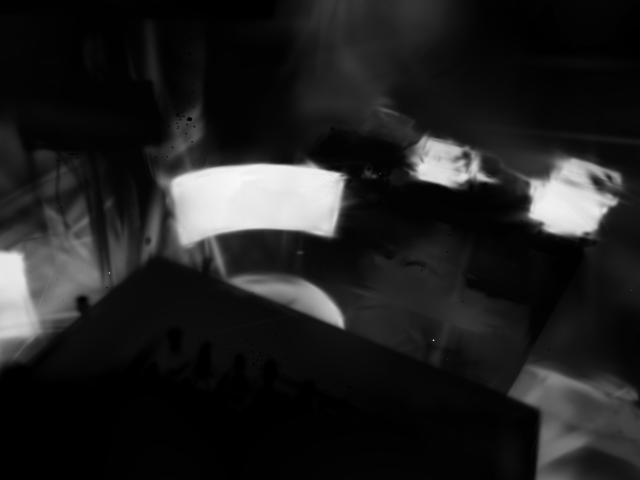
\includegraphics[width=12mm]{fig4/a_vacuity.png}};
\node[sub, anchor=north] at (11.05,-2.90) {rendered $U_r$ (9)};
% temperature chip
\node[mod, draw=outLn, text width=16mm, font=\scriptsize\color{ink}] (temp) at (13.35,-2.45)
  {temperature $\tau$\\(held-out fit)};

% the gold evidence rail
\draw[evflow] (2.1,-2.1) -- node[sym, above=0mm] {$u$} (5.45,-2.35);
\draw[evflow] (6.75,-2.35) -- (8.4,-2.5);
\draw[evflow] (9.95,-2.34) -- node[sym, above=0.6mm, pos=0.45] {$\tilde{u}_i$ per splat} (urimg.west);
\draw[evflow] (urimg.east) -- (temp.west);

% injections: UP into row 1, DOWN into row 2 -- one channel, both bands
\draw[inject] (9.35,-1.95) -- node[sym, right=0.2mm]
  {gate $e^{-\lambda_u(\tilde{u}^G_i+u^q_j)}$} (match.south);
\draw[inject] (10.25,-3.60) -- node[sym, left=0.2mm, pos=0.42, fill=white, inner sep=1pt]
  {$\bar U_r{\le}u_{\max}$} (corr.north);
\draw[inject] (11.65,-3.60) -- node[sym, right=0.2mm, pos=0.42, fill=white, inner sep=1pt]
  {$w{=}e^{-\gamma U_r}$} (refine.north);
\draw[inject] (temp.south) -- node[sym, right=0.2mm] {$\tau$} (lap.north);

% ======================= PANELS (background layer) ==========================
\begin{scope}[on background layer]
  % offline strip
  \node[fill=ink!5, draw=ink!35, dashed, rounded corners=3pt, inner sep=2.6mm,
        fit={(edlhead) (map3d) (-0.20,2.05) (2.55,-3.95)}] (offpan) {};
  % coarse panel
  \node[fill=coarseBg, draw=coarseLn, rounded corners=3pt, inner sep=2.8mm,
        fit={(enc) (match) (hyplab) (13.9,0.2)}] (cpan) {};
  % fine panel
  \node[fill=fineBg, draw=fineLn, rounded corners=3pt, inner sep=2.8mm,
        fit={(corr) (refine) (wimg) (6.75,-7.75)}] (fpan) {};
  % calibrated pose head panel
  \node[fill=poseC!8, draw=poseC!60, rounded corners=3pt, inner sep=2.8mm,
        fit={(lap) (14.6,-6.45) (14.6,-5.25)}] (ppan) {};
  % evidence band
  \node[fill=outBg, draw=outLn!70, rounded corners=3pt, inner sep=2.8mm,
        fit={(5.45,-1.8) (temp) (urimg) (14.3,-3.42) (5.45,-3.42)}] (epan) {};
\end{scope}
\node[panlab, anchor=south west] at (offpan.north west)
  {Offline: evidential mapping (III-A)};
\node[panlab, anchor=south west] at (cpan.north west) {Coarse (IV-B,C)};
\node[panlab, anchor=south west] at (fpan.north west) {Correction + fine (IV-D,E)};
\node[panlab, anchor=south west, color=poseC] at (ppan.north west)
  {Calibrated pose posterior};
\node[panlab, anchor=south west, color=outLn!80!ink] at (epan.north west)
  {One evidential channel: created once, never dropped};

% map feeds the online flow
\draw[flow] (2.18,-0.42) -- node[sym, above=0.4mm, pos=0.62] {$\mathcal{M}$}
  (2.95,-0.42) -- (8.4,-0.42) -- (match.south west);

\end{tikzpicture}
\end{document}
}
  \caption{The \method{} pipeline (reproduced from the letter). Offline, an
  evidential semantic 3DGS map is trained; online, one evidential channel
  gates matching, weights rendering-based refinement, and calibrates the
  output posterior.}
  \label{fig:overview}
\end{figure*}

%------------------------------------------------------------------------------
\section{Implementation Details}
\label{sec:impl}

\subsection{Offline map training}
Each scene is trained by a four-stage pipeline (\texttt{scripts/train\_map.py}
in the released code); Table~\ref{tab:mapcfg} lists every hyperparameter.
Gaussians are initialized by back-projecting the depth maps of every 25th
mapping frame at a stride of 8 pixels, voxel-deduplicated at 2\,cm, and capped
at 200k seeds. The photometric fit uses gsplat rasterization~\cite{kerbl3dgs} with
DefaultStrategy densification, plain RGB colors (no spherical harmonics), and
an L1 loss at $320{\times}240$ for 7{,}000 iterations, one random view per
iteration over every 10th mapping frame. Semantic distillation runs FastSAM~\cite{fastsam}
masks with CLIP~\cite{clip} ViT-B/16 crop embeddings on every 20th frame; each mask's
embedding is accumulated onto the Gaussians whose centres project inside the
mask, pass a depth-occlusion test ($|z-d|<0.15$\,m), and lie in front of the
camera. On chess this yields 330{,}528 Gaussians, of which 94.1\% receive at
least one semantic observation from 9{,}348 mask embeddings; the full
pipeline takes \textbf{94\,s} on an RTX~5070~Ti (16\,GB).

\begin{table}[t]
\caption{Map-training configuration (identical for all scenes).}
\label{tab:mapcfg}
\centering\scriptsize
\setlength{\tabcolsep}{3pt}
\begin{tabular}{@{}lll@{}}
\toprule
Stage & Parameter & Value \\
\midrule
Init & frame / pixel stride & 25 / 8 \\
     & voxel dedup / cap & 2\,cm / 200k \\
Fit  & iterations @ resolution & 7{,}000 @ $320{\times}240$ \\
     & frame stride / loss & 10 / L1 \\
     & densify start--stop / reset & 500--4{,}000 / 3{,}000 \\
     & lr (means$^{*}$, quats, scales) & $1.6{\times}10^{-4*}$, $10^{-3}$, $5{\times}10^{-3}$ \\
     & lr (opacities, colors) & $5{\times}10^{-2}$, $2.5{\times}10^{-3}$ \\
Distill & frame stride / occlusion tol. & 20 / 0.15\,m \\
        & CLIP / segmenter & ViT-B/16 laion2b / FastSAM-s \\
Opinions & full-evidence count $n_0$ & 4 \\
Instances & voxel $\times$ class & 0.4\,m $\times$ argmax class \\
\bottomrule
\multicolumn{3}{@{}l@{}}{\footnotesize $^{*}$scaled by the scene extent, as in 3DGS.}
\end{tabular}
\end{table}

\subsection{Open-vocabulary class set}
The evidential class count is $C{=}25$:
\emph{wall, floor, ceiling, door, window, chair, sofa, table, desk, shelf,
cabinet, monitor, keyboard, mouse, book, cup, bottle, plant, lamp, stairs,
curtain, box, bag, kitchen appliance, sink}. Class prototypes are CLIP text
embeddings of ``\emph{a photo of a $\langle$class$\rangle$ in a room}''.
Pseudo-labels are the argmax cosine similarity, kept only when the
top-1/top-2 margin exceeds 0.01.

%------------------------------------------------------------------------------
\section{The Shared Evidential Head}
\label{sec:edl}

The head is a two-layer MLP ($512 \to 256 \to C$, softplus output,
$\sim$138k parameters, 550\,KB on disk) mapping CLIP features to Dirichlet
evidence. It is trained once, then frozen and shared by the map and query
sides. Neither FastSAM nor CLIP is fine-tuned.

\subsection{Training data and schedule}
\label{sec:edl-training}
The head needs \emph{no manually labeled dataset}: its training set is
generated automatically from the mapping frames themselves during map
building, and Table~\ref{tab:edl-setup} lists the full configuration. Two
feature domains are pooled across ALL scenes (the reasons are Finding~2,
Sec.~\ref{sec:edl-domains}). \emph{Mask domain}: every FastSAM mask crop
embedded by CLIP on the distillation frames of every scene --- 17{,}175
confidence-filtered embeddings over the seven 7Scenes environments (per
scene 504--5{,}375). \emph{Gaussian domain}: the per-Gaussian mask-averaged
features of the already-mapped scenes, subsampled to at most 20k observed
Gaussians per scene --- 23{,}556 after filtering (chess + fire) ---
40{,}731 training features in total. The trained head reaches 70--86\%
pseudo-label agreement on every scene's mask bank with the vacuity ordering
intact. Labels are CLIP zero-shot pseudo-labels: cosine
similarity against the $C{=}25$ text prototypes (``\emph{a photo of a
$\langle$class$\rangle$ in a room}''), argmax kept only when the
top-1/top-2 margin exceeds 0.01; ambiguous features are deliberately
excluded so the head assigns them little evidence at inference, which is
the desired vacuity behavior. Optimization uses the EDL loss~\cite{edl}
(letter, Eq.~7): the Dirichlet Brier risk plus a KL regularizer toward the
uniform Dirichlet on the misleading evidence, annealed as
$\lambda_t = \min(1, \mathrm{epoch}/10)$. Training takes seconds; the head
is then frozen for all scenes and both sides of the pipeline. When a scene
is mapped with a frozen head, stage~4 skips training entirely and only
applies the head.

\begin{table}[t]
\caption{EDL head: complete training configuration (chess numbers).}
\label{tab:edl-setup}
\centering\scriptsize
\setlength{\tabcolsep}{3pt}
\begin{tabular}{@{}ll@{}}
\toprule
Item & Value \\
\midrule
architecture & MLP $512{\to}256{\to}25$, ReLU, softplus \\
parameters / size & $\sim$138k / 550\,KB \\
training set & 40{,}731 CLIP features (auto-generated) \\
\quad mask domain & 17{,}175 crops, ALL 7 scenes \\
\quad Gaussian domain & 23{,}556 sampled (mapped scenes) \\
labels & CLIP zero-shot vs.\ 25 prototypes, argmax \\
label filter & top-1/top-2 cosine margin $> 0.01$ \\
loss & EDL: Brier risk + annealed KL~\cite{edl} \\
KL anneal & $\lambda_t = \min(1, \mathrm{epoch}/10)$ \\
optimizer / lr / batch & Adam / $10^{-3}$ / 512 \\
epochs & 40 (Sec.~\ref{sec:edl-epochs}: why not 10) \\
wall-clock & seconds (RTX 5070 Ti) \\
reuse & trained once, frozen; shared everywhere \\
\bottomrule
\end{tabular}
\end{table}

\subsection{Finding 1: uncertainty structure needs more epochs than accuracy}
\label{sec:edl-epochs}
On a controlled toy problem (4 orthonormal class directions in
$\mathbb{R}^{16}$, 5\% feature noise), classification accuracy exceeds 90\%
within ${\sim}10$ epochs, but the property the vacuity gate relies on ---
\emph{ambiguous inputs earn more vacuity than clean ones} --- is absent at 20
epochs and only emerges by 60 (Table~\ref{tab:edl-epochs}). We therefore
train for 40 epochs by default and regression-test the ordering.

\begin{table}[t]
\caption{Mean vacuity $u$ and top-class belief vs.\ training epochs.
``Mix'' = 50/50 mixtures of two class prototypes (the ambiguous regime);
``junk'' = random unit vectors.}
\label{tab:edl-epochs}
\centering\footnotesize
\setlength{\tabcolsep}{3.5pt}
\begin{tabular}{@{}lcccccc@{}}
\toprule
& \multicolumn{3}{c}{20 epochs} & \multicolumn{3}{c}{60 epochs} \\
\cmidrule(lr){2-4}\cmidrule(lr){5-7}
& clean & mix & junk & clean & mix & junk \\
\midrule
vacuity $u$ & 0.631 & 0.632 & 0.629 & 0.677 & \textbf{0.710} & 0.703 \\
top belief $b_{\max}$ & 0.119 & 0.107 & 0.104 & \textbf{0.223} & 0.136 & 0.111 \\
\bottomrule
\end{tabular}
\end{table}

\subsection{Finding 2: the shared head must train on both input domains}
\label{sec:edl-domains}
The head is applied to raw mask-crop CLIP features (query side) and to
per-Gaussian features averaged over many overlapping masks (map side).
Averaging shifts features off the raw-mask manifold. A head trained only on
mask features assigns the averages near-zero evidence: on chess the median
per-Gaussian vacuity was 0.997 \emph{despite 94\% observation coverage}, and
the primitive-level spread collapsed (Table~\ref{tab:dual-domain}) --- the
gate had nothing to discriminate. Training the same head on the union of both
domains (each pseudo-labeled identically) restores a full spread at no
architectural cost.

The same lesson holds \emph{across scenes}: a dual-domain head trained on
chess alone reached only 8.9\% pseudo-label agreement on fire's features,
and fire's map evidence collapsed exactly as above (median vacuity 0.994).
Pooling the training set over all scenes (Sec.~\ref{sec:edl-training})
restores 70--86\% agreement everywhere. We regard this as a general caution
for shared evidential heads: \emph{share the weights, and share the full
training distribution --- every input domain and every environment the head
will score}.

\begin{table}[t]
\caption{Chess map vacuity with a mask-only vs.\ dual-domain head.
$u_{\mathrm{eff}}$ is the fused primitive-level effective vacuity
(letter, Sec.~IV-A); $q_p$ denotes quantiles.}
\label{tab:dual-domain}
\centering\footnotesize
\setlength{\tabcolsep}{3.5pt}
\begin{tabular}{@{}lcc@{}}
\toprule
 & mask-only head & dual-domain head \\
\midrule
per-Gaussian median $u$ & 0.997 & 0.761 \\
per-Gaussian $q_{10}$ & 0.995 & 0.223 \\
primitive $u_{\mathrm{eff}}$ $q_{10}/q_{25}/q_{50}$ & 0.82 / 0.89 / 0.99 & 0.001 / 0.26 / 0.97 \\
primitives with $u_{\mathrm{eff}}{<}0.7$ & 8 / 1916 & 629 / 1916 \\
primitives with $u_{\mathrm{eff}}{<}0.1$ & 0 / 1916 & 402 / 1916 \\
\bottomrule
\end{tabular}
\end{table}

\subsection{Evidence scaling and fusion behavior}
Per-Gaussian evidence is scaled by observation count,
$e \leftarrow e \cdot \min(1, n/n_0)$ with $n_0{=}4$: a never-observed
Gaussian has $u{=}1$ exactly, and evidence accumulates with support, as
subjective logic prescribes. Note that with $C{=}25$ classes the
\emph{per-observation} vacuity floor is high ($u = C/S$), which is not a
defect: cluster-level DST fusion multiplies member vacuities, so agreement
across members compounds into confidence (the bimodal primitive distribution
of Table~\ref{tab:dual-domain}), while disagreement routes conflict into
vacuity under Yager's rule~\cite{yager,dst}. The absolute scale is absorbed by the gate
sharpness $\lambda_u$ and pixel-weight sharpness $\gamma$; only the ordering
matters, which Sec.~\ref{sec:edl-epochs} verifies.

%------------------------------------------------------------------------------
\section{Evidential Map Statistics}
\label{sec:mapstats}
Table~\ref{tab:mapstats} summarizes the per-scene maps.
\TODO{fill the remaining six scenes after the batch build (plan step 3.1)}

\begin{table}[t]
\caption{Per-scene evidential map statistics (SfM pseudo-GT poses).}
\label{tab:mapstats}
\centering\scriptsize
\setlength{\tabcolsep}{3pt}
\begin{tabular}{@{}lcccccc@{}}
\toprule
Scene & splats & prims & obs. & masks & med $u$ & s \\
\midrule
chess      & 330{,}528 & 1{,}916 & 94.1\% & 9{,}348 & 0.761 & 94 \\
fire       & \res & \res & \res & \res & \res & \res \\
heads      & \res & \res & \res & \res & \res & \res \\
office     & \res & \res & \res & \res & \res & \res \\
pumpkin    & \res & \res & \res & \res & \res & \res \\
redkitchen & \res & \res & \res & \res & \res & \res \\
stairs     & \res & \res & \res & \res & \res & \res \\
\bottomrule
\end{tabular}
\end{table}

%------------------------------------------------------------------------------
\section{Retrieval-Encoder Training on Real Data}
\label{sec:retrieval}

Positive InfoNCE pairs are (FastSAM+CLIP+EDL instances of frames at offsets
$\{0,\pm4,\pm8\}$ around a submap anchor, the submap's reference primitives);
anchors are every 20th mapping frame, and the neighboring frames act as
natural augmentation of the query side.

\subsection{Finding 3: submaps must be frustum-culled}
With radius-only submaps ($r{=}3$\,m) in a room smaller than the radius,
every chess submap contained 768--1{,}529 of the 1{,}916 primitives; all
reference scene descriptors collapsed onto one vector (pairwise cosine
0.9996--1.0000) and the symmetric InfoNCE loss sat exactly at chance,
$\ln(24) \approx 3.178$, for 400 iterations. Culling each submap to the
primitives that project into its anchor view (in front of the camera, inside
the image) yields 154--340 primitives per submap with Jaccard overlap
${\sim}0.40$ between neighboring anchors, and the loss
\TODO{report the converged InfoNCE value and a small loss-curve figure}.
This mirrors the covisibility submaps of SGLoc~\cite{sgloc}: viewpoint content, not a
distance ball, is the retrieval unit.

%------------------------------------------------------------------------------
\section{Extended Evaluation Protocol}
\label{sec:protocol}
All headline numbers follow the letter's protocol; this section fixes the
details a reproduction needs. \textbf{Ground truth}: the SfM
pseudo-GT poses of Brachmann \emph{et al.}~\cite{brachmann2021dslam} for 7Scenes~\cite{sevenscenes_b} and per-scene SfM focal lengths (525.14--527.75); the DSLAM
and SfM references differ by ${\sim}1$\,cm on the same frame, larger than the
gaps separating recent methods, so mixing them is not benign.
\textbf{Hyperparameter tuning}: on a validation split carved from train-side
frames, disjoint from map-fitting and distillation frames; the test split is
evaluated once with frozen settings. \textbf{Temperature}: $\tau$ is fitted
on train-side calibration frames, never on test queries, and the full test
split is reported. \textbf{Seeds}: the Ours and ablation rows are the median
of 3 seeds. \TODO{state the exact validation frame rule and calibration
frame count once frozen (plan steps 2.6 and 3.2)}

%------------------------------------------------------------------------------
\section{Extended Results}
\label{sec:results}

\subsection{Per-scene calibration}
\begin{table}[h]
\caption{Per-scene coverage at nominal 68.3/95.4/99.7\% (tempered), AUSE and
NLL. The letter reports the aggregate; ambiguous scenes (stairs) probe the
Gaussian assumption per hypothesis.}
\label{tab:perscene-calib}
\centering\footnotesize
\setlength{\tabcolsep}{3.5pt}
\begin{tabular}{@{}lccccc@{}}
\toprule
Scene & cov.\ 68.3 & cov.\ 95.4 & cov.\ 99.7 & AUSE$_t$ & NLL \\
\midrule
chess & \res & \res & \res & \res & \res \\
fire & \res & \res & \res & \res & \res \\
heads & \res & \res & \res & \res & \res \\
office & \res & \res & \res & \res & \res \\
pumpkin & \res & \res & \res & \res & \res \\
redkitchen & \res & \res & \res & \res & \res \\
stairs & \res & \res & \res & \res & \res \\
\bottomrule
\end{tabular}
\end{table}

\subsection{Full ablation grid}
\TODO{full grid over: EDL vs softmax head; gate off ($\lambda_u{=}0$);
pixel weight off ($\gamma{=}0$); Dempster vs Yager; $K{=}1$ vs $3$;
raw vs tempered; fixed-scaled covariance baseline --- with bootstrap CIs
(plan steps 3.3 and 3.6)}

\subsection{Robustness sweeps}
\TODO{error AND coverage/NLL vs (a) mapping budget (fit stride 10/40/80),
(b) distillation sparsity (stride 20/80/200), (c) degraded semantics; the
claim under test: accuracy degrades gracefully while calibration holds
(plan step 3.4)}

\subsection{Per-stage runtime}
\TODO{retrieval / refinement / Laplace+condensation ms on RTX 5070 Ti
(plan step 3.5); map training is 94 s/scene (Sec.~\ref{sec:impl})}

%------------------------------------------------------------------------------
\section{DSLAM-Protocol Comparison with SGLoc}
\label{sec:sgloc}
SGLoc~\cite{sgloc} evaluates on 4 of 7 scenes under the original DSLAM ground truth,
which the pseudo-GT study~\cite{brachmann2021dslam} shows to be the easier convention; the letter
therefore keeps this comparison out of Table~I. For completeness:
\TODO{run \method{} under DSLAM GT (omit --sfm-pose-dir) on chess, fire,
heads, office and tabulate against SGLoc's reported numbers}

\begin{table}[h]
\caption{DSLAM-protocol comparison (median cm / deg).}
\label{tab:sgloc}
\centering\small
\begin{tabular}{@{}lcccc@{}}
\toprule
& chess & fire & heads & office \\
\midrule
SGLoc & \res & \res & \res & \res \\
\method{} (ours) & \res & \res & \res & \res \\
\bottomrule
\end{tabular}
\end{table}

%------------------------------------------------------------------------------
\section{Additional Figures}
\label{sec:figs}
\figbox{3.2cm}{\TODO{Fig.: query RGB / rendered vacuity $U_r$ / pixel weight
$w$ triptychs on 2--3 queries (plan step 4.2)}}\par\medskip
\figbox{3.2cm}{\TODO{Fig.: per-query pose-error CDFs vs the strongest
baselines}}\par\medskip
\figbox{3.2cm}{\TODO{Fig.: refinement error vs iteration, with and without
the vacuity pixel weight}}

%------------------------------------------------------------------------------
\section*{Reproducibility}
All numbers in this report regenerate from the released code:
\texttt{train\_map.py} (Sec.~\ref{sec:impl}--\ref{sec:mapstats}),
\texttt{train\_encoders.py} (Sec.~\ref{sec:retrieval}), and
\texttt{run\_7scenes.py} (Sec.~\ref{sec:results}); the per-table commands are
listed in the repository. \TODO{insert repository URL at camera-ready; the
anonymized mirror during review}

\bibliographystyle{IEEEtran}
\bibliography{references}

\end{document}
